%!TEX root = main.tex

\section{Architecture}
\label{sec:arch}

The architecture of the new \ght data-on-demand service consists of two loosely coupled parts:
a web server that handles data requests from users and the \ght server that performs the data extraction.
The two servers communicate via messaging queues.

The interaction between the different subcomponents of the web and \ght servers is illustrated in
Figure~\ref{fig:architecture} and is detailed next.
First, users specify their requests for data by filling in the web form at \url{http://ghtorrent.org/lean} \circled{1}.
A request listener validates each request (e.g., it must contain an email address, it must not ask for
more than 100 repositories)\bv{check number}\as{What happens if the limit is exceeded?}
and records metadata about its owner, payload,\as{What kind of payload do you envision and how does the request listener record it?} 
timestamp and status (completed, in progress) in
a relational database.
Then, for each \gh repository part of the request, the listener posts a message to the queue \circled{2}
containing the request identifier, timestamp and repository.

On the \ght server side, a dispatcher listens in on the requests queue \circled{3} and interprets the
messages received as follows.
First, if the message refers to a request for which no previous messages (asking for different repositories)
have been received, a new shared relational database is created to collect metadata for the repositories part
of this request \circled{4}.
This database has the same schema as the original \ght MySQL database~\cite{gousios2013ghtorent},
reproduced for completeness in Figure~\ref{fig:schema}.
Then, for each message (repository) referring to the same job, a retrieval worker is instantiated having
as parameters the repository being requested, details for connecting to the job database, and the
timestamp of the request \circled{5}.

Retrieval workers run in parallel and make extensive use of caching.
If the main \ght database already contains data for this repository and this data is not too old
(i.e., the difference between the request timestamp and the timestamp of the last update to this data is at
most three months\bv{check number}), then the shared job database is populated with metadata for this
repository extracted from the main \ght database \circled{6}.\as{Would it be a better strategy to allow the 
user to enforce the database repopulation overwriting the cache? in the same way as with the cached webpages?} 
Otherwise, both the main \ght database and the job database \circled{7} are updated with data freshly extracted
from the \gh API.
This data collection process, again designed as a decentralized process, with decentralization mediated
using a similar \emph{worker queue model}, was described previously~\cite{gousios2013ghtorent}.
Once a retrieval worker finishes, it posts a message to the responses queue \circled{8} signalling
the completion of its task.

On the web server side, a response listener handles incoming response messages (one for each repository
in each request) \circled{9} and updates the status of the job in the requests database.
When ``task complete'' messages have been received for all repositories part of a request, data dumps
are being created from both the job database (MySQL, having the \ght schema~\cite{gousios2013ghtorent})
and the main \ght database (MongoDB, only collections---groupings of MongoDB documents---relevant for this
request are extracted).

Finally, the request owner is notified via email that her job has completed and the requested data dumps
are available for download at a given URL.
\as{This all sounds like a good-weather scenario. Should one describe what happens if something is going wrong? For instance,
how do we ensure consistency of the data or what happens if the mail notification bounces? Do we want some kind of
protection of \ght against malicious bots/users that might try to overload \ght servers?}

\begin{figure*}[t]
\begin{center}
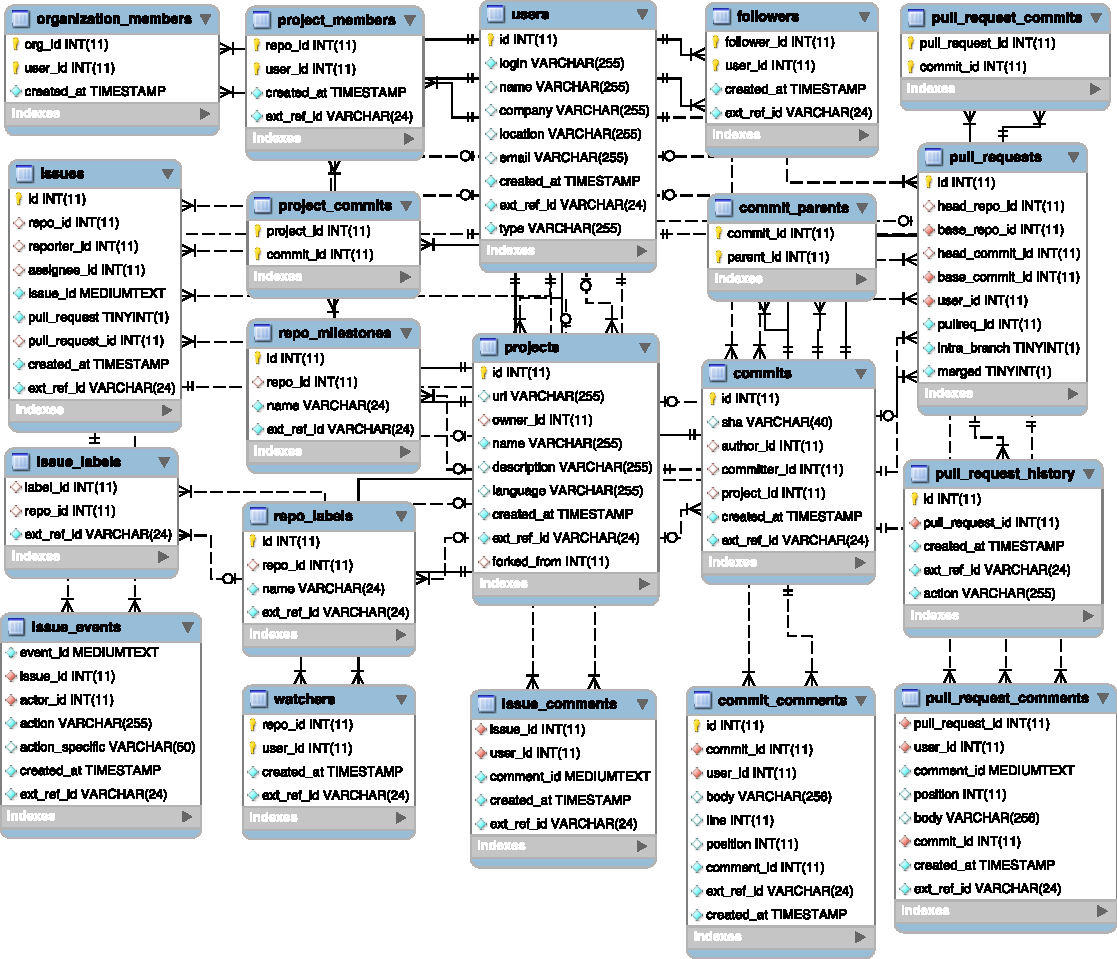
\includegraphics[width=0.9\textwidth]{figures/schema.pdf}
\caption{MySQL database schema~\cite{gousios2013ghtorent}.}
\label{fig:schema}
\end{center}
\end{figure*}

